\documentclass[11pt]{beamer}
\usepackage[utf8]{inputenc}
\usepackage{graphicx, epsfig}
\usepackage{amsmath,mathrsfs,amsfonts,amssymb}
%\usepackage{subfig}
\usepackage{floatflt}
\usepackage{epic,ecltree}
\usepackage{mathtext}
\usepackage{fancybox}
\usepackage{fancyhdr}
\usepackage{multirow}
\usepackage{enumerate}
\usepackage{epstopdf}
\usepackage{multicol}
\usepackage{algorithm}
\usepackage[noend]{algorithmic}
\usepackage{tikz}
\usepackage{blindtext}
\usetheme{default}%{default}%{Singapore}%{Warsaw}%{Warsaw}%{Darmstadt}
\usecolortheme{default}
\setbeamerfont{title}{size=\Huge}
\setbeamertemplate{footline}[page number]{}


\makeatletter
\newcommand\HUGE{\@setfontsize\Huge{35}{40}}
\makeatother    

\setbeamerfont{title}{size=\HUGE}
\beamertemplatenavigationsymbolsempty

% latin bold lower
\newcommand{\ba}{\mathbf{a}} 
\newcommand{\bc}{\mathbf{c}} 
\newcommand{\be}{\mathbf{e}} 
\newcommand{\bh}{\mathbf{h}} 
\newcommand{\bp}{\mathbf{p}} 
\newcommand{\bt}{\mathbf{t}} 
\newcommand{\bs}{\mathbf{s}} 
\newcommand{\bu}{\mathbf{u}} 
\newcommand{\bv}{\mathbf{v}} 
\newcommand{\bw}{\mathbf{w}} 
\newcommand{\bx}{\mathbf{x}} 
\newcommand{\by}{\mathbf{y}} 
\newcommand{\bz}{\mathbf{z}} 

% latin bold upper
\newcommand{\bA}{\mathbf{A}} 
\newcommand{\bB}{\mathbf{B}} 
\newcommand{\bC}{\mathbf{C}} 
\newcommand{\bI}{\mathbf{I}} 
\newcommand{\bL}{\mathbf{L}} 
\newcommand{\bM}{\mathbf{M}} 
\newcommand{\bQ}{\mathbf{Q}} 
\newcommand{\bT}{\mathbf{T}} 
\newcommand{\bU}{\mathbf{U}} 
\newcommand{\bV}{\mathbf{V}} 
\newcommand{\bW}{\mathbf{W}} 
\newcommand{\bX}{\mathbf{X}} 
\newcommand{\bY}{\mathbf{Y}} 
\newcommand{\bZ}{\mathbf{Z}} 

% latin cal upper
\newcommand{\cG}{\mathcal{G}} 
\newcommand{\cL}{\mathcal{L}} 
\newcommand{\cN}{\mathcal{N}} 
\newcommand{\cS}{\mathcal{S}} 
\newcommand{\cT}{\mathcal{T}} 
\newcommand{\cW}{\mathcal{W}} 
\newcommand{\cX}{\mathcal{X}} 
\newcommand{\cZ}{\mathcal{Z}} 

% latin bb upper
\newcommand{\bbE}{\mathbb{E}} 
\newcommand{\bbI}{\mathbb{I}} 
\newcommand{\bbP}{\mathbb{P}} 
\newcommand{\bbR}{\mathbb{R}} 

% greek bold lower
\newcommand{\bepsilon}{\boldsymbol{\epsilon}} 
\newcommand{\btheta}{\boldsymbol{\theta}} 
\newcommand{\blambda}{\boldsymbol{\lambda}} 
\newcommand{\bpi}{\boldsymbol{\pi}} 
\newcommand{\bmu}{\boldsymbol{\mu}} 
\newcommand{\bsigma}{\boldsymbol{\sigma}} 
\newcommand{\bphi}{\boldsymbol{\phi}} 

% greek bold upper
\newcommand{\bSigma}{\boldsymbol{\Sigma}} 

\DeclareMathOperator*{\argmin}{arg\,min}
\DeclareMathOperator*{\argmax}{arg\,max}
\newcommand{\createdgmtitle}[1]{\title[\hbox to 56mm{Mathematical Forecasting Methods \hfill\insertframenumber\,/\,\inserttotalframenumber}]
	{\vspace{1.5\cm} \\ Mathematical Forecasting Methods \\ {\Huge Лекция #1}}
	\author{}
	\institute{
	МФТИ
	} 
	\date{Осень, 2023}
}

\newcommand\myfootnote[1]{%
  \tikz[remember picture,overlay]
  \draw (current page.south west) +(1in + \oddsidemargin,0.5em)
  node[anchor=south west,inner sep=0pt]{\parbox{\textwidth}{%
      \rlap{\rule{10em}{0.4pt}}\raggedright\scriptsize \textit{#1}}};}

\newcommand\myfootnotewithlink[2]{%
  \tikz[remember picture,overlay]
  \draw (current page.south west) +(1in + \oddsidemargin,0.5em)
  node[anchor=south west,inner sep=0pt]{\parbox{\textwidth}{%
      \rlap{\rule{10em}{0.4pt}}\raggedright\scriptsize\href{#1}{\textit{#2}}}};}
\setbeamertemplate{blocks}[rounded]
\setbeamercolor{block title}{bg=beamer@blendedblue!25, fg=beamer@blendedblue}
\setbeamercolor{block body}{bg=beamer@blendedblue!10}
\usepackage{graphicx,animate}
% \usepackage{xmpmulti}


\setbeamercolor{block title alerted}{bg=red!25, fg=red}
\setbeamercolor{block body alerted}{bg=red!10}
\createdgmtitle{8}
\usepackage{tikz}
\usepackage{amsmath}
\usepackage[english,russian]{babel}
\usepackage[labelformat=empty]{caption}

\usepackage{graphicx,animate}
\usepackage{animate}
\usepackage{svg}
\usepackage{subcaption}

\usetikzlibrary{arrows,shapes,positioning,shadows,trees}
\newcommand*{\defeq}{\stackrel{\text{def}}{=}}

%--------------------------------------------------------------------------------
\begin{document}
%--------------------------------------------------------------------------------
\begin{frame}[plain]
%\thispagestyle{empty}
\titlepage
\end{frame}

\begin{frame}{RNN и метод Эйлера}
    Рассмотрим рекуррентные модели:
    \begin{displaymath}
        \bh_{t+1} = \bh_t + f(\bh_t, \btheta),
    \end{displaymath}
    где $t\in \{1, \dots, T\}$. \par
    Можно заметить что данная формула эквивалентна дискретизации обыкновенных ДУ методом Эйлера при $\Delta t = 1$
    \begin{displaymath}
        \bh(t+1) = \bh(t) + f(\bh(t), t, \btheta) \Rightarrow f(\bh(t), t, \btheta) = \frac{\bh(t+1) - \bh(t)}{\Delta t}
    \end{displaymath}
    Т.о. если мы в пределе возьмем больше слоев с меньшим шагом, мы получим непрерывную динамики праметризированную обычной нейронной сетью
    \begin{displaymath}
        \frac{d\bh(t)}{dt} = f(\bh(t), t, \btheta).
    \end{displaymath}
\end{frame}

\begin{frame}{Обобщение}
    Таким образом RNN аппроксимирует функцию динамики  с помощью метода Эйлера.  Однако мы не ограничены только этим методом. На самом деле мы можем взять любой (нарпимер метод Рунге-Кутты). \par
    \begin{block}{}
    Пусть $\bx = \bh(t_0)$ - начальное значение и $\by = \bh(t_1)$ - конечное значение, тогда
    \begin{displaymath}
        \by = \int_{t_0}^{t_1}f(\bh(t), t, \btheta)dt + \bx = ODESolve(\bx, f, t_0, t_1, \btheta)
    \end{displaymath}
    \end{block}
    
    Теперь чтобы обновить параметры $\btheta$ необходимо взять градиент скалярной функции потерь $\cL(\by)$ по параметрам $\frac{\partial\cL(\by)}{\partial \btheta}$\par
    \begin{alertblock}{\textbf{Проблема}}
        Если воспользоваться бэкпропом то потребуется больших затрат памяти, т.к. будем проходить по операциям солвера.
    \end{alertblock}
    
\end{frame}

\begin{frame}{Neural ODE}
    Для этого введем сопряженное (adjoint) состояние, которое показывает как изменяется функция потерь от скрытого состояния $\bh(t)$ в некоторый момент $t$:
    \begin{displaymath}
            \ba_\bh(t) = \frac{\partial \cL(\by)}{\partial \bh(t)}
    \end{displaymath}
    и динамика которого задается следующим ДУ:
    \begin{block}{Теорема Понтрягина (часть 1)}
        \begin{displaymath}
            \frac{d\ba_\bh(t)}{dt} = -\ba_\bh(t)\frac{\partial f(\bh(t), t, \btheta)}{\partial \bh(t)} = g(\bh(t), t)
        \end{displaymath}
    \end{block}
    Соответственно чтобы получить сопряженное состояние в момент $t_0$ мы таже можем запустить солвер из $t_1$ в $t_0$:
    \begin{displaymath}
        \begin{split}
            \ba_\bh(t_0) = -\int_{t_1}^{t_0}\ba_\bh(t)\frac{\partial f(\bh(t), t, \btheta)}{\partial \bh(t)}dt + \frac{\partial \cL(\by)}{\partial \by} = \\ = ODESolve(\by, g, t_1, t_0, \btheta)
        \end{split}
    \end{displaymath}
    \myfootnotewithlink{https://arxiv.org/abs/1806.07366}{Chen R. T. Q. et al. Neural Ordinary Differential Equations, 2018}
\end{frame}

\begin{frame}{Neural ODE}
    Теперь, когда мы можем посчитать сопряженное состояние для любого момента $t$, получим градиент по параметрам:
    \begin{displaymath}
        \ba_{\btheta}(t_0) = \frac{\partial\cL(\by)}{\partial \btheta},
    \end{displaymath}
    динамика которого задается следующим ДУ:
    \begin{block}{Теорема Понтрягина (часть 2)}
        \begin{displaymath}
            \frac{d\ba_{\btheta}(t)}{dt} = -\ba_\bh(t)\frac{\partial f(\bh(t), t, \btheta)}{\partial \btheta} = g'(\ba_\bh(t), \bh(t), t)
        \end{displaymath}
    \end{block}
    Соответственно чтобы получить сопряженное состояние в момент $t_0$ мы таже можем запустить солвер из $t_1$ в $t_0$:
    \begin{displaymath}
        \begin{split}
            \ba_{\btheta}(t_0) = -\int_{t_1}^{t_0}\ba_\bh(t)\frac{\partial f(\bh(t), t, \btheta)}{\partial \btheta}dt + {\color{violet}0} = \\ = ODESolve(\by, g', t_1, t_0, \btheta)
        \end{split}
    \end{displaymath}
    \myfootnotewithlink{https://arxiv.org/abs/1806.07366}{Chen R. T. Q. et al. Neural Ordinary Differential Equations, 2018}
\end{frame}

\begin{frame}{Neural ODE}
    По полученным выражениям заметно, что для того чтобы посчитать сопряженное состояние  $\ba_\bh(t)$ требуется знать скрытое состояние $\bh(t)$, а для градиета по параметрам $\ba_{\btheta}(t)$ необходимо знать оба вышеперечисленных значения. Таким образом обучение Neural ODE следует по следующей схеме
    \begin{block}{Forward pass}
        \begin{displaymath}
        \by = ODESolve(\bx, f, t_0, t_1, \btheta)
    \end{displaymath}
    \end{block}
    \begin{block}{Backward pass}
        \begin{displaymath}
            \begin{cases} 
                \ba_{\btheta}(t_0) = ODESolve(\by, g', t_1, t_0, \btheta)
                \\ 
                \ba_\bh(t_0) = ODESolve(\by, g, t_1, t_0, \btheta)
                \\
                \bx = ODESolve(\by, f, t_1, t_0, \btheta)
            \end{cases}
        \end{displaymath}
    \end{block}
    \myfootnotewithlink{https://arxiv.org/abs/1806.07366}{Chen R. T. Q. et al. Neural Ordinary Differential Equations, 2018}
\end{frame}

\begin{frame}{Neural ODE}
    Для того чтобы не вызывать несколько раз солвер на этапе \textit{backward pass} можно конкатенировать все три вектора $\ba_{\btheta}(t)$, $\ba_\bh(t)$ и $\bh(t)$ и вызвать по ним \textit{только один} солвер
    \begin{figure}
            \centering
            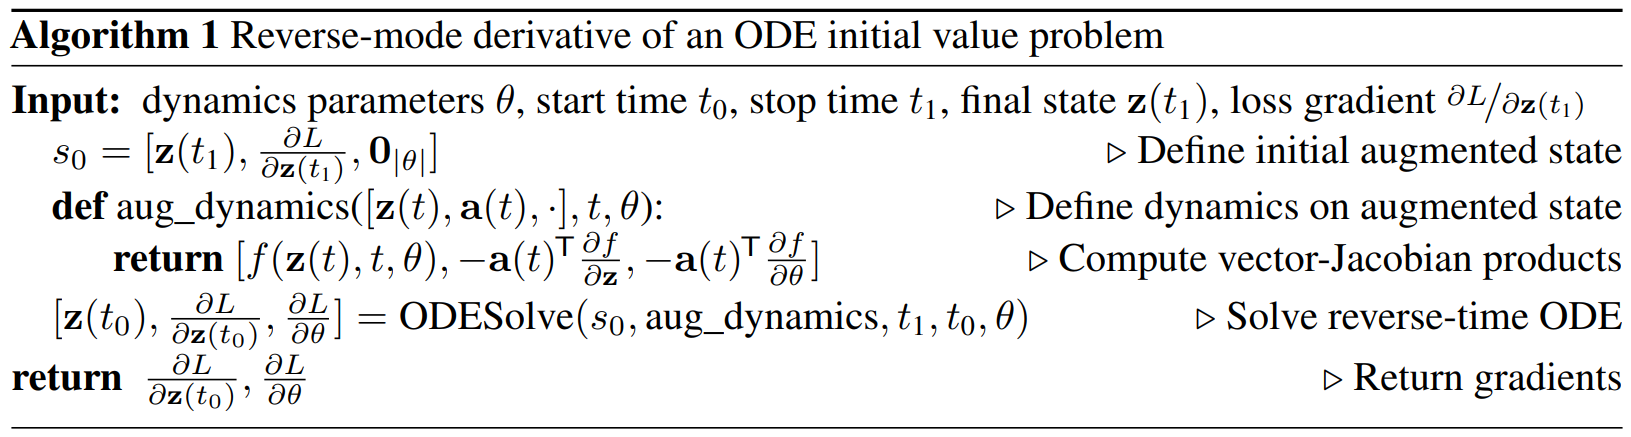
\includegraphics[width=0.85\linewidth]{figures/alg.png}
            \label{fig:alg}
        \end{figure}
    \myfootnotewithlink{https://arxiv.org/abs/1806.07366}{Chen R. T. Q. et al. Neural Ordinary Differential Equations, 2018}
\end{frame}

\begin{frame}{Neural ODE}
    Теперь если нам необходимо знать градиенты для разных моментов $t_i$ $\forall i\in\{1,\dots, N\}$ в forward pass мы получаем значение $h(t_i)$. Этап backward pass мы разбиваем на пары $(t_i, t_{i+1})$ и применяем для каждой солвер. Далее каждое сопряженное состояние $\ba_\bh(t_i)$ мы смещаем на соответсвенный градиент $\frac{\partial \cL(\bh(t_{i+1}))}{\partial \bh(t_i)}$
    \begin{figure}
        \centering
        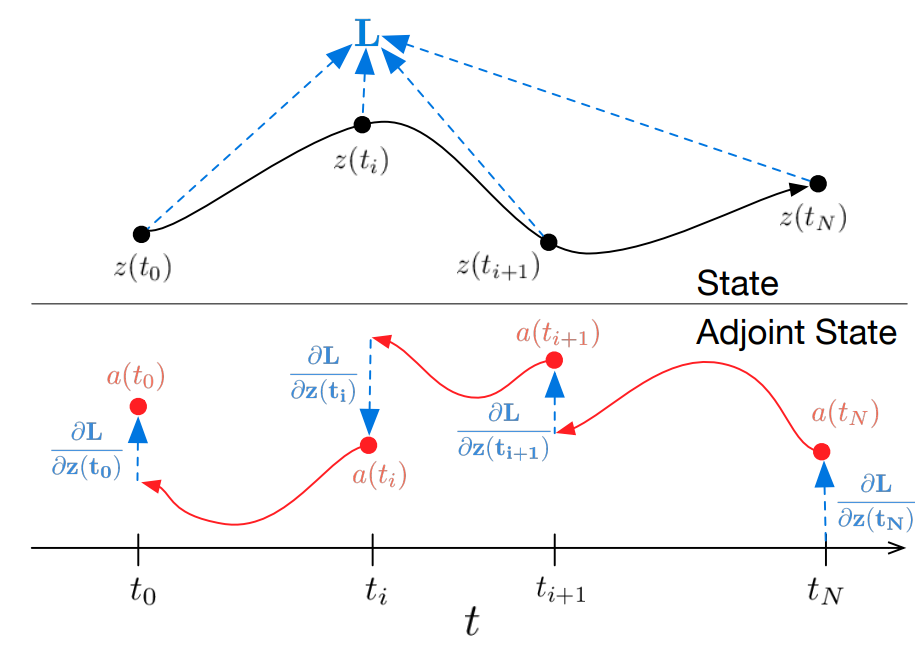
\includegraphics[width=0.6\linewidth]{figures/reverse.png}
        \label{fig:rev}
    \end{figure}
    \myfootnotewithlink{https://arxiv.org/abs/1806.07366}{Chen R. T. Q. et al. Neural Ordinary Differential Equations, 2018}
\end{frame}

\begin{frame}{Выводы}
    \begin{itemize}
        \item \textbf{Модели непрерывных временных рядов}: В отличие от рекуррентных нейронных сетей, которые требуют дискретизации интервалов наблюдения, Neural ODE позволяет работать с данными, полученными с \textit{произвольными} временными интервалами
        \item \textbf{Непрерывные нормализующие потоки}: Неожиданным побочным преимуществом непрерывных преобразований является то, что формула замены переменных становится легче вычислять
    \end{itemize}

\end{frame}

\begin{frame}{Пример}
    % \transduration<0-25>{0.2}
    % \multiinclude[<+->][format=jpg, graphics={width=\textwidth}]{frame}
    \begin{figure}
        \centering
        \animategraphics[width=\textwidth, loop, autoplay, autoplay controls=all]{10}{figures/frame-}{0}{25}
    \end{figure}
    \myfootnotewithlink{https://habr.com/ru/companies/ods/articles/442002/}{Михаил Сурцуков, Знакомство с Neural ODE, 2019}
\end{frame}

\end{document} 